\documentclass[
 pdftex, 
 oneside, % Einseitiger Druck.
 12pt, % Schriftgroesse
 parskip=half, % Halbe Zeile Abstand zwischen Absätzen.
 headsepline, % Linie nach Kopfzeile.
 %footsepline, % Linie vor Fusszeile.
 abstracton % Abstract Überschriften
%  ngerman % Translator
]{scrreprt}  
 
%Seitenränder:
\usepackage[ 
	top=25mm, 
	left=30mm, 
	right=25mm, 
	bottom=32mm,
	headsep=10mm, 
	footskip=15mm
	]{geometry} 
	
\usepackage{lscape}
	

%Seite von oben bis unten füllen und ggf. Abstände minimalst dehnen	

%\usepackage{fullpage} %Seitengroesse
\usepackage[activate]{microtype} %Zeilenumbruch und mehr

% Zeichencodierung:
\usepackage[T1]{fontenc}
\usepackage[utf8]{inputenc}
  
\usepackage[onehalfspacing]{setspace} % Zeilenabstand
\usepackage{makeidx} % Index-Erstellung
\usepackage[ngerman]{babel} % Lokalisierung (neue deutsche Rechtschreibung)
\usepackage[babel,german=quotes]{csquotes} % deutsche Anführungszeichen

\usepackage{graphicx} % Grafiken
%Grafiken immer im selben Kapitel einfügen wo sie referenziert werden
\usepackage{placeins} 

% einfachere Querverweise mit Seitenangabe usw.:
\usepackage{prettyref}
\newrefformat{cha}{Kapitel~\ref{#1} auf Seite~\pageref{#1}}  % Für Kapitel 
\newrefformat{sec}{Abschnitt~\ref{#1} auf Seite~\pageref{#1}} % Für Abschnitte
\newrefformat{fig}{Abbildung~\ref{#1} auf Seite~\pageref{#1}}% Für Abbildungen
\newrefformat{tab}{Tabelle~\ref{#1} auf Seite~\pageref{#1}}	 % Für Tabellen
\newrefformat{lst}{Quellcode~\ref{#1} auf Seite~\pageref{#1}} % für Quellcodeliings 

 
%merhspaltige Elemente möglich machen
\usepackage{multicol} 

%Mathe-Zeugs und Text-Anordnung
\usepackage{amsmath}
\usepackage{amssymb} 

%serifenlose Schriftart:
\renewcommand{\familydefault}{\sfdefault}
\usepackage{sfmath}

\usepackage{float}
\restylefloat{table}
   
% Spezielle Tabellenform fuer Deckblatt
\usepackage{longtable}
\setlength{\tabcolsep}{10pt} %Abstand zwischen Spalten
\renewcommand{\arraystretch}{1.5} %Zeilenabstand

% Farben
\usepackage{color}
\definecolor{LinkColor}{rgb}{0,0,0.5}
\definecolor{ListingBackground}{rgb}{0.92,0.92,0.92}

%Farben in Tabellen nutzen
\usepackage{colortbl}
\definecolor{light-gray}{gray}{0.80}

\clubpenalty=10000
\widowpenalty=10000
\displaywidowpenalty=10000 

% Quellcode
\usepackage{listings}
\usepackage{scrhack} %bessere Integration in KOMA-Script, Warning wegbekommen
\definecolor{javared}{rgb}{0.6,0,0} % for strings
\definecolor{javagreen}{rgb}{0.25,0.5,0.35} % comments
\definecolor{javapurple}{rgb}{0.5,0,0.35} % keywords
\definecolor{javadocblue}{rgb}{0.25,0.35,0.75} % javadoc

\lstset{
	language=Java, % Sprache des Quellcodes
	numbers=left, % Zelennummern links
	stepnumber=1, % Jede Zeile nummerieren.
	numbersep=5pt, % 5pt Abstand zum Quellcode
	lineskip=1pt, % Zeilenabstand im Quellcode
	numberstyle=\tiny, % Zeichengrösse 'tiny' für die Nummern.
	breaklines=true, % Zeilen umbrechen wenn notwendig.
	breakautoindent=true, % Nach dem Zeilenumbruch Zeile einrücken.
	postbreak=\space, % Bei Leerzeichen umbrechen.
	tabsize=2, % Tabulatorgrösse 2
	basicstyle=\ttfamily\footnotesize, % Nichtproportionale Schrift, klein für den Quellcode
	showspaces=false, % Leerzeichen nicht anzeigen.
	showstringspaces=false, % Leerzeichen auch in Strings ('') nicht anzeigen.
	%basicstyle=\ttfamily, 
	morekeywords={var, function},
	keywordstyle=\color{javapurple}\bfseries,
	stringstyle=\color{javared},
	commentstyle=\color{javagreen},
	morecomment=[s][\color{javadocblue}]{/**}{*/},
	backgroundcolor=\color{ListingBackground}, % Hintergrundfarbe des Quellcodes
	% setzen.
	captionpos=b, % sets the caption-position to bottom
	%extendedchars=true, % Alle Zeichen vom Latin1 Zeichensatz anzeigen.
    literate={ö}{{\"o}}1 %deutsche Sonderzeichen auch in Listings
    		 {Ö}{{\"O}}1 %funktionierend machen durch escapen
         	 {Ü}{{\"U}}1
         	 {ü}{{\"u}}1
         	 {Ä}{{\"A}}1
         	 {ä}{{\"a}}1
         	 {ß}{{\ss}}1
}
\renewcommand{\lstlistlistingname}{Quellcodeverzeichnis}
\renewcommand{\lstlistingname}{Quellcode}

%Glossar-Einträge konfigurieren:
\usepackage[
	nonumberlist, %keine Seitenzahlen anzeigen
	%acronym,      %ein separates Abkürzungsverzeichnis erstellen
	toc,          %Einträge im Inhaltsverzeichnis
	section]      %im Inhaltsverzeichnis auf section-Ebene erscheinen
{glossaries}
\glsenablehyper   %Abkürzungen ins Glossar verlinken
\renewcommand*{\glspostdescription}{} %Punkt nach Beschreibung deaktivieren

%Wort aus Glossar bei erster Verwendung hervorheben
\defglsdisplayfirst{\emph{#1}} 
\defglsdisplayfirst[acronym]{\emph{#1}} 
 
 
%Literaturverzeichnis formatieren
\bibliographystyle{plaindin} %Literaturverzeichnis nach DIN-Norm darstellen
  
% Verschiedene Schriftarten
%\usepackage{goudysans}
%\usepackage{lmodern}
%\usepackage{libertine}
\usepackage{palatino} 


\newcommand{\pdftitel}{\autor \space \arbeit \space \semester}
\newcommand{\pdfsubject}{\arbeit \space \semester}
\newcommand{\autor}{Ephraim Petry \& Nick Herrmannsdörfer}
\newcommand{\arbeit}{Studienarbeit}
\newcommand{\semester}{Semester 5 + 6}


\newcommand{\titel}{Entwicklung einer Lern-Feedback-Plattform für Vorlesungen}
\newcommand{\subtitel}{Lecture Monitoring - LeMon}
\newcommand{\martrikelnrEphraim}{2767400}
\newcommand{\martrikelnrNick}{1655361}
\newcommand{\kurs}{TINF11D}
\newcommand{\datumAbgabe}{06. Juni 2014}
\newcommand{\abschluss}{Bachelor of Science}
\newcommand{\studiengang}{Informatik}
\newcommand{\vertiefung}{Angewandte Informatik}
\newcommand{\dhbw}{Stuttgart} 
\newcommand{\betreuer}{Frau Dr. Barbara Dörsam}
\newcommand{\zeitraum}{zwei Semester}
\newcommand{\abgabeort}{Stuttgart}

% Titel, Autor und Datum
\title{\titel}
\author{\autor}
\date{\datum}
 
%URl-Umbrüche auch an Bindestrichen für lange URLs erlauben
 \usepackage[hyphens]{url}
% set colors for links and URLs und URLs nicht escapen
\usepackage[
	colorlinks=true, 
    urlcolor=blue,
    linkcolor=black,
    citecolor=black,
    filecolor=black,
    %menuecolor=black,
    pdftitle={\pdftitel},
	pdfauthor={\autor},
	pdfsubject={\pdfsubject},
	pdfcreator={pdflatex, LaTeX with KOMA-Script},
	pdfpagemode=UseOutlines, % Beim Oeffnen Inhaltsverzeichnis anzeigen
	pdfdisplaydoctitle=true, % Dokumenttitel statt Dateiname anzeigen.
	pdflang=de % Sprache des Dokuments.
	]{hyperref} % Hyperlinks als solche machen

% Fußnoten
\usepackage[
	perpage, %Fußnoten-Nummerierung auf jeder Swite neu beginnen
	hang,	 %Abstand zwischen Zahl und Text in der Fußnote 
	multiple, 
	stable]  %Fußn. in Überschriften anzeigen, aber nicht im Inhaltsverzeichnis
{footmisc}


\usepackage{fancyhdr}


 \pagestyle{fancy}{
 	 	\newcommand{\clearHeader}{\fancyhead{}\fancyfoot{}}
	\fancyhead{}
	\fancyfoot{}  	
 	\fancyfoot[C]{\thepage}
	\fancyhead[L]{
\includegraphics[height=0.65cm]{images/dhbw-Logo.png}}
 	
 
 	\fancyhead[C]
 	{
 	 \begin{tabular}[b]{l}
 	  LeMon
 	 \end{tabular}
 	}

 %	\fancyhead[R]
 %	{
 %	 \begin{tabular}[b]{l}
 %	  \includegraphics[height=1.3em]{images/IBM-Logo.png}\\
 %	 \end{tabular}
 %	}
 	
 	\newcommand{\emptyHeader}{
 	\fancyhead{}
 	\fancyfoot{}
 	\renewcommand{\headrulewidth}{0pt}
 	}

 }
\fancypagestyle{plain}{
	 	\newcommand{\clearHeader}{\fancyhead{}\fancyfoot{}}
	\fancyhead{}
	\fancyfoot{}  	
 	\fancyfoot[C]{\thepage}
	\fancyhead[L]{
\includegraphics[height=0.65cm]{images/dhbw-Logo.png}}
 	
 
 	\fancyhead[C]
 	{
 	 \begin{tabular}[b]{l}
 	  LeMon
 	 \end{tabular}
 	}

 %	\fancyhead[R]
 %	{
 %	 \begin{tabular}[b]{l}
 %	  \includegraphics[height=1.3em]{images/IBM-Logo.png}\\
 %	 \end{tabular}
 %	}
 	
 	\newcommand{\emptyHeader}{
 	\fancyhead{}
 	\fancyfoot{}
 	\renewcommand{\headrulewidth}{0pt}
 	}

}
\fancypagestyle{abstract}{
	 	\newcommand{\clearHeader}{\fancyhead{}\fancyfoot{}}
	\fancyhead{}
	\fancyfoot{}  	
 	\fancyfoot[C]{\thepage}
	\fancyhead[L]{
\includegraphics[height=0.65cm]{images/dhbw-Logo.png}}
 	
 
 	\fancyhead[C]
 	{
 	 \begin{tabular}[b]{l}
 	  LeMon
 	 \end{tabular}
 	}

 %	\fancyhead[R]
 %	{
 %	 \begin{tabular}[b]{l}
 %	  \includegraphics[height=1.3em]{images/IBM-Logo.png}\\
 %	 \end{tabular}
 %	}
 	
 	\newcommand{\emptyHeader}{
 	\fancyhead{}
 	\fancyfoot{}
 	\renewcommand{\headrulewidth}{0pt}
 	}

}
%Abkürzungen
%
% Abkürzungen --> referenz, name, beschreibung
% Aufruf mit \gls{...} oder Kurzform mit \acrshort{...}

\newacronym{DHBW}{DHBW}{Duale Hochschule Baden Württemberg}
\newacronym{HDM}{HDM}{Hochschule der Medien}
\newacronym{LeMon}{LeMon}{Lecture Monitoring}
\newacronym{HTML}{HTML}{Hypertext Markup Language}
\newacronym{SQL}{SQL}{Standard Query Language}
\newacronym{Ajax}{Ajax}{Asynchronous JavaScript and XML}

\newglossaryentry{PHP}{name={PHP}, first={PHP}, description={Hypertext Preprocessor, eine Skriptsprache zur serverseitigen Programmierung und Verarbeitung von Webinhalten}}
\newglossaryentry{adoDB}{name={adoDB}, first={adoDB}, description={Ein Framework zum Kapseln der Zugriffe auf Datenbanken}}
\newglossaryentry{jQuery}{name={jQuery}, first={jQuery}, description={Eine JavaScript-Bibliothek zum Manipulieren von browserübergreifenden DOM-Objekten}}
\newglossaryentry{PHPQRCode}{name={PHPQRCode}, first={PHPQRCode}, description={Eine PHP Library zur Erzeugung von 2-dimensionalen Barcodes (sogenannten QR-Codes)}}
\newglossaryentry{pChart}{name={pChart}, first={pChart}, description={Eine PHP Library zur Erzeugung von Diagrammen}}
\newglossaryentry{JavaScript}{name={JavaScript}, first={JavaScript}, description={JavaScript ist eine Script-Sprache zur Clientseitigen Programmierung}}
\newglossaryentry{Bootstrap}{name={Bootstrap}, first={Bootstrap}, description={Bootstrap ist eine JavaScript Bibliothek}}

\newglossaryentry{IDE}{name={IDE}, first={Integrated development environment
(IDE)}, description={Integrated development environment / Integrierte
Entwicklungs-Umgebung}}



% 	\newcommand{\clearHeader}{\fancyhead{}\fancyfoot{}}
	\fancyhead{}
	\fancyfoot{}  	
 	\fancyfoot[C]{\thepage}
	\fancyhead[L]{
\includegraphics[height=0.65cm]{images/dhbw-Logo.png}}
 	
 
 	\fancyhead[C]
 	{
 	 \begin{tabular}[b]{l}
 	  LeMon
 	 \end{tabular}
 	}

 %	\fancyhead[R]
 %	{
 %	 \begin{tabular}[b]{l}
 %	  \includegraphics[height=1.3em]{images/IBM-Logo.png}\\
 %	 \end{tabular}
 %	}
 	
 	\newcommand{\emptyHeader}{
 	\fancyhead{}
 	\fancyfoot{}
 	\renewcommand{\headrulewidth}{0pt}
 	}


%Glossar-Befehle anschalten
\makeglossaries

%%%%%%%%%%%%%%%%%%%%%%%%%%%%%%%%%%%%%%%%%%%%%%%%%%%%%%%%%%%%%%%%%%%%%%%%%%%%%%%%


\begin{document} 

\cleardoublepage{}
 
% Deckblatt 
\begin{titlepage}
\begin{longtable}{p{.55\textwidth} p{.85\textwidth}}
%{\includegraphics[height=2.6cm]{images/IBM-Logo.png}} &
{
\includegraphics[height=2.6cm]{images/dhbw-Logo.png}}
\end{longtable}
\enlargethispage{20mm}
\begin{center}
\vspace*{8mm} {\LARGE \bf \titel }\\
\vspace*{3mm} {\Large\bf \subtitel} \\
\vspace*{12mm} {\large \bf \arbeit}\\
\vspace*{12mm} {\large \bf \semester}\\
  
\vspace*{12mm} Studiengang  \textit{\studiengang\\}
\vspace*{5mm} Vertiefungsrichtung \textit{\vertiefung\\}
\vspace*{9mm} an der \linebreak Dualen Hochschule Baden-Württemberg / \dhbw\\
\vspace*{12mm} von\\ 
\vspace*{3mm} {\large\bf \autor}\\
\vspace*{12mm} \datumAbgabe\\
\end{center}
\vfill
\begin{spacing}{1.2}
\begin{tabbing}
mmmmmmmmmmmmmmmnmmmmmmmmmmmm \= \kill
\textbf{Bearbeitungszeitraum} \> \zeitraum\\
\textbf{Matrikelnummer Ephraim Petry, Kurs} \> \martrikelnrEphraim, \kurs\\
\textbf{Matrikelnummer Nick Herrmannsdörfer, Kurs}\> \martrikelnrNick, \kurs\\
\textbf{Betreuer der Praxisphase} \> \betreuer\\
\end{tabbing}
\end{spacing}
\end{titlepage}
\thispagestyle{empty}

\begin{flushleft}
\begin{spacing}{1.2}
\begin{tabbing}
mmmmmmmmmmmmmmmnmmnmm \= \kill
\textbf{Name}: \> \autor \\
\textbf{Matrikel-Nr Ephraim Petry}: \> \martrikelnrEphraim\\
\textbf{Matrikel-Nr Nick Herrmannsdörfer}: \> \martrikelnrNick\\
\textbf{Kurs}: \> \kurs \\
\end{tabbing}
\end{spacing}



\vspace{1em}
\textbf{Titel der Arbeit:} \linebreak \titel: \newline \subtitel

\end{flushleft}
\vspace*{4em}

\section*{Erklärung}
\vspace*{1em}

Ich versichere hiermit, dass ich das vorliegende Dokument selbständig verfasst und keine
anderen als die angegebenen Quellen und Hilfsmittel verwendet habe.

\vspace{1em}
\begin{flalign*}
\text{\abgabeort, \datumAbgabe} \hspace{5mm}
%\rule{_Breite_}{_Stärke_} %%andersrum ist's vertikal;)
& \rule{0.7\textwidth}{0.5pt} \notag\\
& \autor \notag
\end{flalign*} 

\renewcommand{\abstractname}{Zusammenfassung}
\begin{abstract} 
 
Im Rahmen dieser Studienarbeit sollte ein System erstellt werden, mit dem der Lernfortschritt und
das Verständnis  der Studenten an der \gls{HDM} für die in der Vorlesung vermittelten Inhalte
abgeprüft werden sollte. Dieses System sollte \gls{LeMon} heißen.

Das System sollte dabei den kompletten Prozess von der Erstellung einzelner Übungsblätter durch den
Dozenten, das Management der Fragen für die Übungsbläter, sowie das Freischalten der Übungsblätter
zur entsprechenden Zeit beinhalten.
Desweiteren sollte der Dozent den Studenten auf einfache Art und Weise das elektronische Übungsblatt
zugänglich machen. Hierzu sollte bevorzugt ein QR-Code eingesetzt werden, den die Studenten mit
ihrem Smartphone und einer entsprechenden App sofort einlesen und zum Übungsblatt gelangen konnten.
\newline Am Ende sollte der Dozent auf einfache Weise die Möglichkeit haben, die Ergebnisse wenige
Sekunden nach Ablauf der Zeit anschaulich angezeigt zu bekommen und diese mit den Studenten
durchsprechen.

Zur Umsetzung dieses Projektes sollte eng mit einer Gruppe mit einem ähnlichen Projekt
zusammengearbeitet werden, die jedoch eine etwas andere Art von Übungsblättern für den Einsatz von
Aufgaben innerhalb oder auch außerhalb der Vorlesung erstellen sollte. Soweit möglich sollten dabei
Synergien genutzt und eine gemeinsame Oberfläche für beide Projekte erstellt werden.




 
 \end{abstract} 
\chapter*{Vorwort}
Dies ist die Studienarbeit von Ephraim Petry und Nick Herrmansdörfer. Sie ist bestandteil des
dritten Studienjahres des Bachelor-Studiums an der \gls{DHBW} Stuttgart.

Diese Studienarbeit sollte nicht nur den Zweck der Absolvierung einer Studienarbeit erfüllen. Ein
besonderes Augenmerk lag auch darauf, dass bestehende oberflächliche Wissen in bestimmten
Technologien in als praktisches Projekt umzusetzen und zu vertiefen.

\glsresetall
\renewcommand{\baselinestretch}{1.50}\normalsize
%\chapter*{Vorwort}
Dies ist die Studienarbeit von Ephraim Petry und Nick Herrmansdörfer. Sie ist bestandteil des
dritten Studienjahres des Bachelor-Studiums an der \gls{DHBW} Stuttgart.

Diese Studienarbeit sollte nicht nur den Zweck der Absolvierung einer Studienarbeit erfüllen. Ein
besonderes Augenmerk lag auch darauf, dass bestehende oberflächliche Wissen in bestimmten
Technologien in als praktisches Projekt umzusetzen und zu vertiefen.

\tableofcontents 
\glsresetall 
\chapter{Einleitung}

Im Rahmen dieser Studienarbeit sollte ein System erstellt werden, mit dem der Lernfortschritt und
das Verständnis  der Studenten an der \gls{HDM} für die in der Vorlesung vermittelten Inhalte
abgeprüft werden sollte. Dieses System sollte \gls{LeMon} heißen.

Das System sollte dabei den kompletten Prozess von der Erstellung einzelner Übungsblätter durch den
Dozenten, das Management der Fragen für die Übungsbläter, sowie das Freischalten der Übungsblätter
zur entsprechenden Zeit beinhalten.
Desweiteren sollte der Dozent den Studenten auf einfache Art und Weise das elektronische Übungsblatt
zugänglich machen. Hierzu sollte bevorzugt ein QR-Code eingesetzt werden, den die Studenten mit
ihrem Smartphone und einer entsprechenden App sofort einlesen und zum Übungsblatt gelangen konnten.
\newline Am Ende sollte der Dozent auf einfache Weise die Möglichkeit haben, die Ergebnisse wenige
Sekunden nach Ablauf der Zeit anschaulich angezeigt zu bekommen und diese mit den Studenten
durchsprechen.

Zur Umsetzung dieses Projektes sollte eng mit einer Gruppe mit einem ähnlichen Projekt
zusammengearbeitet werden, die jedoch eine etwas andere Art von Übungsblättern für den Einsatz von
Aufgaben innerhalb oder auch außerhalb der Vorlesung erstellen sollte. Soweit möglich sollten dabei
Synergien genutzt und eine gemeinsame Oberfläche für beide Projekte erstellt werden.


\section{Aufgabenstellung}

 

% Hier könnte eine Einleitung stehen \emph{Hervorgehoben} \cite{LiteraturEintrag1}
% 
% \section{Überschrift abc}
% Abcdef ghijklmno pqrstuvw xyz äöü\ldots \gls{DHBW}
%  
% \section{Überschrift abcd}\label{sec:Ueberschriftabcd}
% Abcdef ghijklmno pqrstuvw xyz ÄÖÜ\ldots 
% 
% \prettyref{sec:Ueberschriftabcd}
% 
% 
% \begin{figure} [!htb]
% 	\begin{center}
% 		  \begin{tabular}{@{}r@{}}
% 		{
\includegraphics[width=14cm]{images/dhbw-Logo.png}}\\
% 		\footnotesize\sffamily\textbf{Quelle:} DHBW-Homepage
% 	  		   \cite{LiteraturEintrag1}
%  	 	 \end{tabular} 	
% 		\caption{Das DHBW-Logo}
% 		\label{fig:DHBWLogo}
% 	\end{center} 
% \end{figure}
\chapter{Anforderungsanalyse} 
\section{Use-Cases} \label{sec:Use-Cases}

% %Ideen für Spacing:
% %\itemsep -5pt
% %Vorlage:
% \begin{table}[h]
% 	\begin{tabular}{|p{3cm}|p{11.06cm}|}
% 	\hline
% 		\multicolumn{2}{|l|}{\textbf{UC Nr.} }   \\ \hline
% 		\textbf{Name}                 &         \\ \hline
% 		\textbf{Ziel im Kontext}      &         \\ \hline
% 		\textbf{Akteure}              &         \\ \hline
% 		\textbf{Trigger}              &         \\ \hline
% 		\textbf{Essenzielle Schritte} & 
% 			\begin{enumerate}
% 			  \item sdf
% 			  \item 
% 			\end{enumerate}
% 		\\ \hline
% 		\textbf{Erweiterungen} 		  &         \\ \hline
% 	\end{tabular}
% \end{table}\FloatBarrier
% 
% \begin{table}[h]
% 	\begin{tabular}{|p{3cm}|p{11.06cm}|}
% 	\hline
% 		\textbf{Zugehöriger Use Case}                 &         \\ \hline
% 		\textbf{Beteiligte Tabellen}      &         \\ \hline
% 		\textbf{Vorbedingung}              &         \\ \hline
% 		\textbf{Ablauf}              &   
% 			\begin{enumerate}
% 			  \item sdf
% 			  \item 
% 			\end{enumerate}
% 		\\ \hline
% 		\textbf{Erweiterungen}              &         \\ \hline
% 	\end{tabular}
% \end{table}\FloatBarrier

\begin{table}[h] 
\subsection{UC1: Frage mit Musterlösungen anlegen}\label{uc:UC1}
	\begin{tabular}{|p{3cm}|p{11.06cm}|}
	\hline
		\multicolumn{2}{|l|}{\textbf{UC Nr.: UC1} }   \\ \hline
		\textbf{Name}                 &      Frage mit Musterlösungen anlegen   \\ \hline
		\textbf{Ziel im Kontext}      &      Dozent legt eine neue Frage mit ihrer Musterlösung an   \\ \hline
		\textbf{Akteure}              &      Dozent (D.)   \\ \hline
		\textbf{Trigger}              &      D. klickt auf "`Frage anlegen"'   \\ \hline
		\textbf{Essenzielle Schritte} & 			
			\begin{enumerate}
			  \item D. befindet sich im Admin Bereich
			  \item D. klickt auf „Frage anlegen“
			  \item D. sieht Web Interface zum Frage erstellen
			  \item	D. wählt den Fragentyp aus einer Auswahlmöglichkeit aus
			  \item D. wählt die Kategorie für die Frage aus einer Auswahlmöglichkeit aus
			  \item D. gibt Frage in das dazu passende Feld ein
			  \item D. gibt die zur Frage passende/n Musterlösung/en in das/die passende/n Feld/er ein
			  \item D. klickt abschließend auf „Abschicken“
			\end{enumerate}			
		\\ \hline
		\textbf{Erweiterungen} 		  &   4a. D. gibt an wie viele Antworten für Aufzählaufgaben gefordert werden     \\ \hline
	\end{tabular}
	\caption{Use Case 1: Frage mit Musterlösungen anlegen}
\end{table}\FloatBarrier




\begin{table}
\subsection{UC2: Kategorie anlegen}\label{uc:UC2}
	\begin{tabular}{|p{3cm}|p{11.06cm}|}
	\hline
		\multicolumn{2}{|l|}{\textbf{UC Nr.: UC2} }   \\ \hline
		\textbf{Name}                 &     Kategorie anlegen   \\ \hline
		\textbf{Ziel im Kontext}      &     Dozent legt eine neue Kategorie an   \\ \hline
		\textbf{Akteure}              &     Dozent (D.)    \\ \hline
		\textbf{Trigger}              &     D. klickt auf „Kategorie anlegen“    \\ \hline
		\textbf{Essenzielle Schritte} & 
			\begin{enumerate} 
			  \item D. befindet sich im Admin Bereich
			  \item D. klickt auf „Kategorie anlegen“
			  \item D. sieht Web Interface zum Kategorien erstellen
			  \item D. gibt den Namen der Kategorie in das dazu passende Feld ein
			  \item	D. klickt abschließend auf den „Plus“-Button
			\end{enumerate}
		\\ \hline
		\textbf{Erweiterungen} 		  &         \\ \hline
	\end{tabular}
	\caption{Use Case 2: Kategorie anlegen}
\end{table}\FloatBarrier



\begin{table}[h]
\subsection{UC3: Vorlesung anlegen}\label{uc:UC3}
	\begin{tabular}{|p{3cm}|p{11.06cm}|}
	\hline
		\multicolumn{2}{|l|}{\textbf{UC Nr.: UC3} }   \\ \hline
		\textbf{Name}                 &     Vorlesung anlegen    \\ \hline
		\textbf{Ziel im Kontext}      &     Dozent legt eine neue Vorlesung an   \\ \hline
		\textbf{Akteure}              &     Dozent (D.)    \\ \hline
		\textbf{Trigger}              &     D. klickt auf „Vorlesung anlegen“    \\ \hline
		\textbf{Essenzielle Schritte} & 
			\begin{enumerate}
			  \item D. befindet sich im Admin Bereich
			  \item D. klickt auf „Vorlesung anlegen“
			  \item D. sieht Web Interface zum Vorlesungen anlegen
			  \item D. gibt den Namen der Vorlesung in das dazu passende Feld ein
			  \item D. klickt abschließend auf den „Plus“-Button
			\end{enumerate}
		\\ \hline
		\textbf{Erweiterungen} 		  &         \\ \hline
	\end{tabular}
	\caption{Use Case 3: Vorlesung anlegen}
\end{table}\FloatBarrier



\begin{table}[h]
\subsection{UC4: Arbeitsblatt anlegen}\label{uc:UC4}
	\begin{tabular}{|p{3cm}|p{11.06cm}|}
	\hline
		\multicolumn{2}{|l|}{\textbf{UC Nr.: UC4} }   \\ \hline
		\textbf{Name}                 &     Arbeitsblatt anlegen    \\ \hline
		\textbf{Ziel im Kontext}      &     Dozent legt ein neues Arbeitsblatt an    \\ \hline
		\textbf{Akteure}              &     Dozent (D.)    \\ \hline
		\textbf{Trigger}              &     D. klickt auf „Arbeitsblatt anlegen“    \\ \hline
		\textbf{Essenzielle Schritte} & 
			\begin{enumerate}
			  \item D. befindet sich im Admin Bereich
			  \item D. klickt auf „Arbeitsblatt anlegen“
			  \item D. sieht Web Interface zum Erstellen eines Arbeitsblattes
			  \item D. gibt den Namen des Arbeitsblattes in das dazu passende Feld ein
			  \item D. erhält Übersicht aller Fragen mit Checkbox zum Auswählen mit Filtermöglichkeit
			  \item D. sieht eine extra Tabelle mit den bisher ausgewählten Fragen
			  \item D. klickt nach Hinzufügen aller gewünschten Fragen auf „Arbeitsblatt anlegen“, wenn alle gewünschten Fragen hinzugefügt wurden
			\end{enumerate}
		\\ \hline
		\textbf{Erweiterungen} 		  &   6a. D. kann die Reihenfolge der Fragen verändern oder sie wieder entfernen      \\ \hline
	\end{tabular}
	\caption{Use Case 4: Arbeitsblatt anlegen}
\end{table}\FloatBarrier




\begin{table}[h]
\subsection{UC5: Antworten abschicken}\label{uc:UC5}
	\begin{tabular}{|p{3cm}|p{11.06cm}|}
	\hline
		\multicolumn{2}{|l|}{\textbf{UC Nr.: UC5} }   \\ \hline
		\textbf{Name}                 &     Antworten abschicken    \\ \hline
		\textbf{Ziel im Kontext}      &     Studenten schicken Antworten ab    \\ \hline
		\textbf{Akteure}              &     Student (S)    \\ \hline
		\textbf{Trigger}              &     S. klickt auf „Antworten abschicken“    \\ \hline
		\textbf{Essenzielle Schritte} & 
			\begin{enumerate}
			  \item S. befindet sich im Studenten-Bereich
			  \item S. klickt auf „Antworten abschicken“
			  \item S. sieht Bestätigungsdialog
			  \item S. klickt auf „OK“
			  \item S. sieht Bestätigungsdialog
			\end{enumerate}
		\\ \hline
		\textbf{Erweiterungen} 		  &   4a. S. klickt auf "`Abbrechen"' und schickt somit seine Antworten noch nicht ab     \\ \hline
	\end{tabular}
	\caption{Use Case 5: Antworten abschicken}
\end{table}\FloatBarrier




\begin{table}[h]
\subsection{UC6: Auswertung des Übungsblattes}\label{uc:UC6}
	\begin{tabular}{|p{3cm}|p{11.06cm}|}
	\hline
		\multicolumn{2}{|l|}{\textbf{UC Nr.: UC6} }   \\ \hline
		\textbf{Name}                 &     Auswertung des Arbeitsblattes    \\ \hline
		\textbf{Ziel im Kontext}      &     Dozent wertet Arbeitsblatt aus   \\ \hline
		\textbf{Akteure}              &     Dozent (D)    \\ \hline
		\textbf{Trigger}              &     D. klickt auf „Auswertung“    \\ \hline
		\textbf{Essenzielle Schritte} & 
			\begin{enumerate}
			  \item D. befindet sich im Admin-Bereich
			  \item D. klickt auf „Auswertung“
			  \item D. sieht Übersicht der verschiedenen Vorlesungen und Arbeitsblättern
			\end{enumerate}
		\\ \hline
		\textbf{Erweiterungen} 		  &         \\ \hline
	\end{tabular}
	\caption{Use Case 6: Auswertung des Übungsblattes}
\end{table}\FloatBarrier

 

\section{Allgemeine Anforderungen}
Die an das Projekt gestellten Anforderungen gliedern sich in zwei Gebiete:
Technologische Anforderungen und allgemeine Anforderungen, die an die
Applikation gestellt werden. Soweit möglich sollte bei der Datenhaltung
Synergie-Effekte mit dem Projekt "`CCKE"' benutzt werden. Ebenso sollte der
Bereich für Lehrbeauftragte für die Erstellung und Verwaltung und Präsentation
der Ergebnisse weit möglichst für beide Projekte einheitlich gehalten werden.

\section{Technologische Anforderungen}
Die zu entwickelnde Applikation sollte auf Basis von Webtechnologien aufgebaut
werden. Desweiteren sollte das Backend für Lehrbeauftragte sowie die Auswertung
der Ergebnisse an einem Notebook bedient werden können. Die Oberfläche für die
Auswertung der Antworten sollte dabei so optimiert sein, dass die Ergebnisse
ohne größeren Aufwand mittels einem im Raum vorhandenen Beamer präsentiert
werden können.  \newline
Die Oberfläche für die Eingabe der Antworten der Studenten sollte dabei für
mobile Geräte optimiert werden, was insbesondere Smartphones und Tablets
beinhalten sollte. Die Optimierung für mobile Geräte sollte die Bedienbarkeit
für verbreitete mobile Platformen sicherstellen. \newline
Die gesamte Datenhaltung der Applikation sollte mit Hilfe einer frei verfügbaren
Datenbank realisiert werden. 

\section{Eingesetzte Technologien}
Bei der Auswahl der Technologien wurde insbesondere Wert darauf gelegt, dass die
Grundlagen für diese den Studenten bereits bekannt sind. Allerdings sollten auch
neue Aspekte unter  zuhilfenahme moderner Ansätze und Frameworks erlernt und so
die Grundlage für eine spätere Erweiterung des Projekts durch nachfolgende
Gruppen sichergestellt werden.

Nachfolgend eine Auflistung der eingesetzten Technologien:
\begin{singlespacing}
  \begin{multicols}{3}
\begin{itemize}
  \item HTML
  \item CSS
  \item JavaScript
  \item AJAX
  \item PHP
  \item SQL
\end{itemize}
\end{multicols}
\end{singlespacing}
\chapter{Vorüberlegungen}
Zu Beginn der Studienarbeit mussten einige Vorüberlegungen getätigt werden:
\begin{itemize}
  \item Es musste ein Datenmodell erstellt werden, welches die Struktur der Datenbank beschreibt.
  \item Es mussten alle zu diesem Zeitpunkt bereits bekannten Aufgaben festgehalten werden, um sich
  einen Überblick über den Funktionsumfang und Arbeitsaufwand zu verschaffen.
\end{itemize}
Aus den so erhaltenen Aufgaben und den Funktionalitäten, die das Projekt am Ende bieten sollte, sollte ein Konzept zum Design einer passenden Oberfläche erstellt werden. 

\section{Datenmodell}
Das Datenmodell wurde früh entwickelt und sollte als Grundlage dienen, um die Datenstruktur der Datenbank implementieren. 
Dabei ist es wichtig Zeit in das Datenmodell zu investieren, da das Datenmodell als fundamentale Grundlage dient und große Änderungen daran später zeitaufwändige Folgen haben würden.
Dabei wurde ein eine relationale Datenbank gewählt und versucht, das Datenmodell nach den Prinzipien der Theorie der realtionalen Datenbanken aufzubauen.
Dementsprechend wurde die Tabellenstruktur in dritter Normalform aufgebaut.\\
Im Verlauf der Studienarbeit mussten dennoch Änderungen am Datenmodell vorgenommen werden, jedoch waren diese nur kleine Änderungen, wie z.B. das Hinzufügen einer Spalte innerhalb einer Tabelle.
Dies lässt den Schluss zu, dass die zu Beginn investierte Zeit in das Datenmodell und die Gespräche und Diskussionen zu Beginn hierzu sinnvoll investierte Zeit waren.

\begin{landscape}
\begin{figure} [!htb]
	\begin{center}
		  \begin{tabular}{@{}r@{}}
			{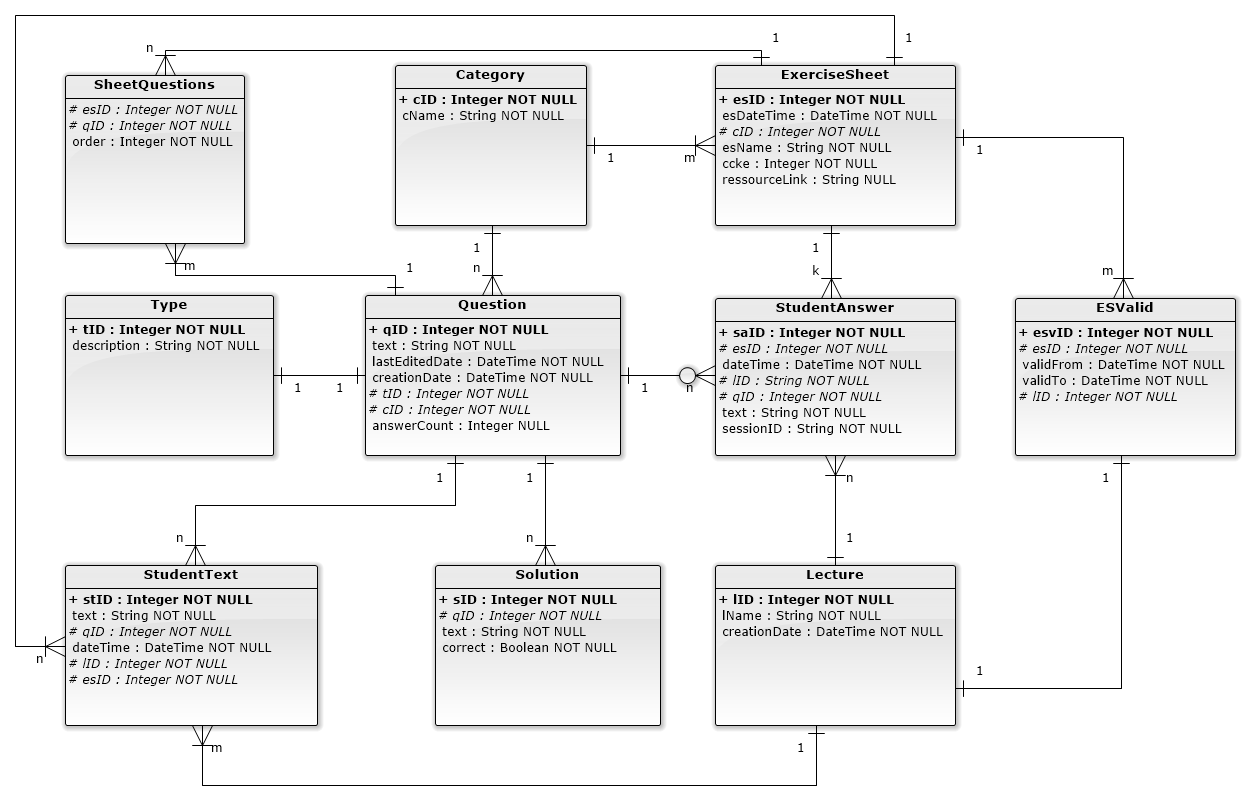
\includegraphics[height=37em]{images/Entityrelationshipdiagram.png}}\\
 	 	 \end{tabular}
		\caption{Datenmodell LeMon + CCKE}
		\label{fig:Datenmodell}
	\end{center} 
\end{figure}

\end{landscape}

\section{Funktionsumfang}
Der letztendliche Funktionsumfang war zu Beginn des Projektes zwar grob klar, wie in Projekten in Unternehmen war es jedoch auch so, dass sich der Kunde gewisse Dinge später anders vorgestellt hat oder gar neue Wünsche für Funktionen äußerte.
Darauf muss man dynamisch agieren und neue Dinge während der Projektphase hinzufügen oder bestehende gegebenenfalls zu überarbeiten.
Für die wichtigsten Funktionalitäten des Projektes, wurden Use-Cases aufgestellt.

\section{Benutzeroberfläche}
Anhand der gesammelten Anforderungen hinsichtlich Funktionalitäten, wurden einige Oberflächen schon weitestgehend definiert. 
Als Beispiel sei hier die Funktion 'Frage erstellen' genannt, bei der gewisse Eingabefelder vorgegeben warem um den Fragentyp und -text festzulegen.
Die letztendlichen Anordnungen wurden dann in direkten Gesprächen mit dem Kunden geklärt.
\chapter{Implementierung}

\section{Struktur des Projekts}
Die Struktur des Projekts auf Datei-Ebene im Ordner \emph{Management} ist folgender
Maßen aufgebaut:

\begin{singlespacing}
	\begin{itemize}
		\item Im Unterordner \emph{Admin} liegen alle Dateien für den Admin-Bereich
		\item Im Unterordner \emph{Frameworks} liegen alle Frameworks die im Projekt verwendet werden
		\item Im Unterordner \emph{Images} liegen alle Bilder und Icons die im Projekt verwendet werden 
		\item Im Unterordner \emph{User} liegen alle Dateien des User-Bereiches
		\item Im Ordner \emph{Management} selbst liegt die \emph{generalConfig.php} Datei, die
		globale Variablen anlegt welche Pfade oder Informationen über die Datenbank
		definiert
	\end{itemize}
\end{singlespacing}


\section{Admin-Bereich}
Der Admin-Bereich ist die Oberfläche über die der Dozent die Möglichkeit hat
neue Fragen, Kategorien, Vorlesungen und Arbeitsblätter zu erstellen.



\subsection{Struktur der Implementierung}
Die Struktur des Admin Bereichs auf Datei-Ebene im Ordner \emph{Admin} ist
folgender Maßen aufgebaut:

\begin{singlespacing}
	\begin{itemize}
		\item Im Unterordner \emph{adminStyles} liegen alle CSS Dateien für den Admin-Bereich
		\item Im Unterordner \emph{js} liegen alle JavaScript Dateien und Bibliotheken für den
		Admin-Bereich
		\item Im Ordner \emph{Admin} selbst liegen alle \gls{PHP} Dateien der einzelnen Unterseiten 
		des Admin-Bereichs
	\end{itemize}
\end{singlespacing}


Die Struktur des Admin Bereichs auf Code-Ebene kann unter dem Begriff der
"`prozeduralen Programmierung"' zusammengefasst werden. Wo dies sinnvoll war, wurden dabei
Funktionen geschrieben die bestimmte Aufgaben abdecken. Durch eine starke
Verzahnung von \gls{PHP} und \gls{HTML} Code und um die Übersichtlichkeit zu gewährleisten, wurde
der \gls{HTML} Code größtenteils mit in den \gls{PHP} Code integriert.


\subsection{Eingesetzte Libraries und Frameworks}
Es werden mehrere Frameworks verwendet um die Funktionalität des Admin-Bereichs
zu erhalten.
\begin{singlespacing}
	\begin{itemize}
	  	\item Mit dem Framework \gls{adoDB}\footnote{AdoDB-Projektseite auf Sourceforge: \url{http://adodb.sourceforge.net}} können Verbindungen mit Datenbank erstellt und gemanaged. Außerdem
			stellt es Funktionen für \gls{SQL} Querys zur Verfügung.
		\item Die bekannte Bibliothek \gls{jQuery}\footnote{JQuery-Projektseite: \url{http://jquery.com}} wird im Admin-Bereich zur Sicherstellung der Crossbrowser-Funktionalität eingesetzt.
		\item Die Bibliothek \gls{PHPQRCode}\footnote{PHPQRCode-Projektseite auf Sourceforge: \url{http://phpqrcode.sourceforge.net}} wird dazu verwendet um QR-Codes durch \gls{PHP} zu
			generieren.
		\item Die Bibliothek \gls{pChart}\footnote{pChart-Projektseite auf Sourceforge: \url{http://pchart.sourceforge.net}} wird zum Erstellen von Auswertungsdiagrammen verwendet.
	\end{itemize}
\end{singlespacing}
 


\subsection{Besonderheiten der Implementierung}
Im Folgenden sollen einige Besonderheiten der Implementierung dargestellt und
erläutert werden.
\begin{singlespacing}
	\begin{itemize}
		\item Damit die Webseite nicht bei jedem Seitenwechsel in der Navigationsleiste
			neu geladen werden muss, wurde zur Navigation Ajax verwendet. Dadurch wird immer
			nur der Seitenbereich mit neuem Content aktualisiert, der Rest der Seite muss
			deswegen nicht unnötig nach geladen werden.
		\item Der QR-Code wird mit der \gls{PHPQRCode} Bibliothek generiert. Dabei ist
			jedoch eine Besonderheit zu beachten: Da der QR-Code nicht unnötig
			zwischengespeichert werden sollte, musste ein besonderes Konstrukt verwendet
			werden. Dabei wird durch eine seperate \gls{PHP} Datei der QR-Code erzeugt und in
			dieser Datei gleichzeitig der Content-Type auf \emph{image/png} gesetzt.
			Anschliesend wird diese \gls{PHP} Datei mit dem generierten Bild in den Image-Tag
			einer anderen Seite eingebettet.
		\item Zur Auswertung von Aufzählaufgaben wird versucht eine möglichst genaue
			Korrektheitsüberprüfung durchzuführen. Dazu werden die gegebenen Antworten der
			Studenten in Kleinbuchstaben konvertiert, Umlaute durch (ae, ue, oe, ss) ersetzt
			und bestimmte Sonderzeichen entfernt. Danach werden diese Antworten mit der nach
			den selben Methoden konvertierten Musterlösung verglichen.
		\item Nach Abschluss des Auswertungsvorganges werden die zu einer Frage
			gehörenden Studentenantworten in einem Diagramm, welches mit der Bibliothek
			\gls{pChart} erstellt wird, dargestellt. In diesem Diagramm sind die Antworten
			grafisch dargestellt.
	\end{itemize}
\end{singlespacing}



\section{LeMon-Bereich}
Der \gls{LeMon}-Bereich begrenzt sich auf das Ausfüllen der für \gls{LeMon} angelegte Arbeitsblätter.
\subsection{Struktur der Implementierung}
Um die Implementierung einfach und übersichtlich zu halten, wurde nach dem Stil
dem Konzept der objektorientierten Programmierung vorgegangen.\\
Folgendermaßen wurde dabei die Ordnerstruktur aufgebaut:

\begin{singlespacing}
	\begin{itemize}
		\item Im Unterordner \emph{css} liegen alle CSS Dateien für den \gls{LeMon}-Bereich
		\item Im Unterordner \emph{image} liegen alle Bilder und Icons, die im
			\gls{LeMon}-Bereich verwendet werden
		\item Im Unterordner \emph{include} liegt zum einen eine PHP Datei, welche die
			Datenbankverbindung sicherstellt und zum anderen eine PHP Datei die zentral alle
			verwendeten Klassen aus dem extra Unterordner \emph{Classes} einbindet.
		\item Im Unterordner \emph{js} liegen alle \gls{JavaScript} Dateien und Bibliotheken für den
			\gls{LeMon}-Bereich
		\item Im Ordner \emph{LeMon} selbst liegt die Arbeitsblatt \gls{PHP} Datei, welche das Layout des Arbeitsblattes festlegt.
	\end{itemize}
\end{singlespacing}


\subsection{Eingesetzte Libraries und Frameworks}
Es werden mehrere Frameworks verwendet um die Funktionalität des LeMon-Bereichs
zu erhalten.
\begin{singlespacing}
	\begin{itemize}
		\item Mit dem Framework \gls{Bootstrap}\footnote{Bootstrap-Projektseite:
			\url{http://getbootstrap.com}}, welches \emph{"`das bekannteste Framework zum Entwickeln
			von responsive mobile first Web-Projekten ist"'} \cite{BootstrapDefinition}, wird
			der LeMon-Bereich auf gängigen Mobilgeräten angepasst dargestellt.
		\item Die bekannte Bibliothek \gls{jQuery}\footnote{JQuery-Projektseite:
			\url{http://jquery.com}} wird im Admin-Bereich zur Sicherstellung der
			Crossbrowser-Funktionalität eingesetzt.
	\end{itemize}
\end{singlespacing}

\section{Benutzeroberfläche}
In diesem Abschnitt werden die Aufgaben der unterschiedlichen Oberflächen kurz
erklärt. Es gibt drei Hauptoberflächen: den \emph{Administrationsbereich}, die
\emph{Ansicht für Studenten} und die \emph{Auswertung}.

\subsection{Administrationsbereich}
In diesem Bereich hat der Dozent die Möglichkeit verschiedene administrative
Aufgaben zu tätigen. Dazu zählen die Funktionen \emph{Fragen anlegen und
verwalten}, \emph{Kategorien anlegen und verwalten}, \emph{Vorlesungen anlegen
und verwalten} und \emph{Arbeitsblätter anlegen und verwalten}.
Im folgenden Screenshot ist zu sehen wie der Administrationsbreich aufgebaut
ist. Im Oberen Bereich der Seite gibt es einen Header mit dem Logo der \gls{HDM},
dazu gibt es im unteren Bereich einen Footer in dem es einen Link zur
Webseite der \gls{HDM} gibt. Auf der linken Seite gibt es eine Navigationsbar über
die es möglich ist zu den einzelnen Funktionen zu navigieren. Rechts-mittig ist
der Bereich in dem die einezlenen Unterformulare der Funktionen angezeigt
werden. 

\begin{figure} [!htb]
	\begin{center}
		  \begin{tabular}{@{}r@{}}
			{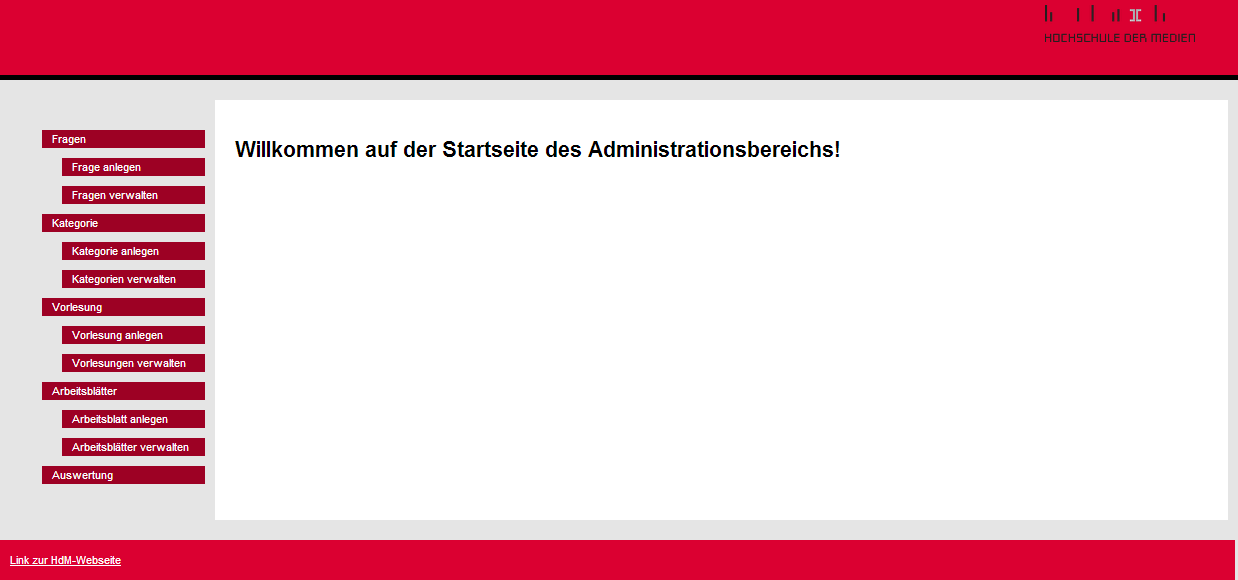
\includegraphics[width=36.6em]{images/Administrationsbereich.png}}\\
 	 	 \end{tabular}
		\caption{Ansicht des Administrationsbereiches}
		\label{fig:Administrationsbereich}
	\end{center} 
\end{figure}\FloatBarrier



\subsection{Ansicht für Studenten}
Diesen Bereich bekommen Studenten zu sehen, wenn sie Aufgabenblätter bearbeiten
sollen. Es werden hier die Fragen für ein bestimmtes Arbeitsblatt aufgelistet.
Die Studenten können das Ausgabenblatt ausfüllen und das Formular abschicken
oder alle Eingabefelder leeren.

\begin{figure} [!htb]
	\begin{center}
		  \begin{tabular}{@{}r@{}}
			{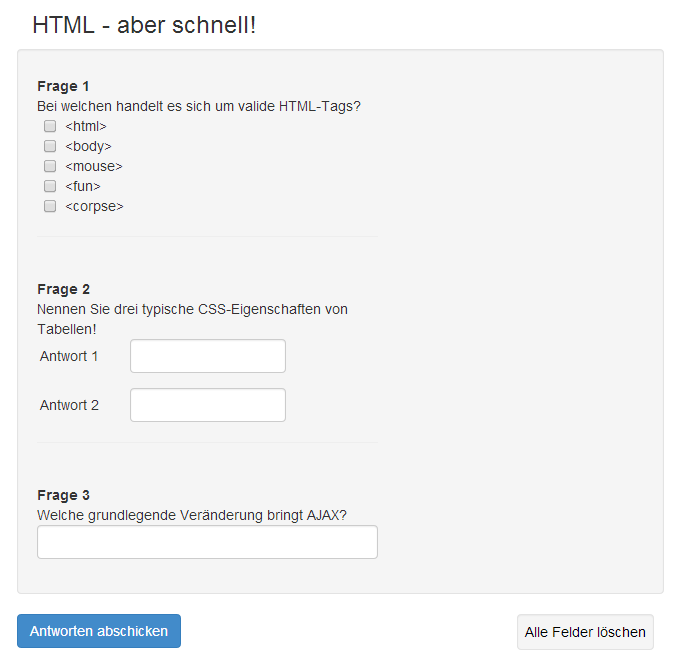
\includegraphics[width=36.6em]{images/Studentenansicht.png}}\\ 
 	 	 \end{tabular}
		\caption{Ansicht für Studenten}
		\label{fig:Studentenansicht}
	\end{center} 
\end{figure}\FloatBarrier

\subsection{Auswertung}
In dem Bereich der Auswertung werden zu einer ausgewählten Vorlesung und einem
Arbeitsblatt die dazugehörigen beantworteten Fragen in Diagrammen oder
Textfelder dargestellt.

\begin{figure} [!htb]
	\begin{center}
		  \begin{tabular}{@{}r@{}}
			{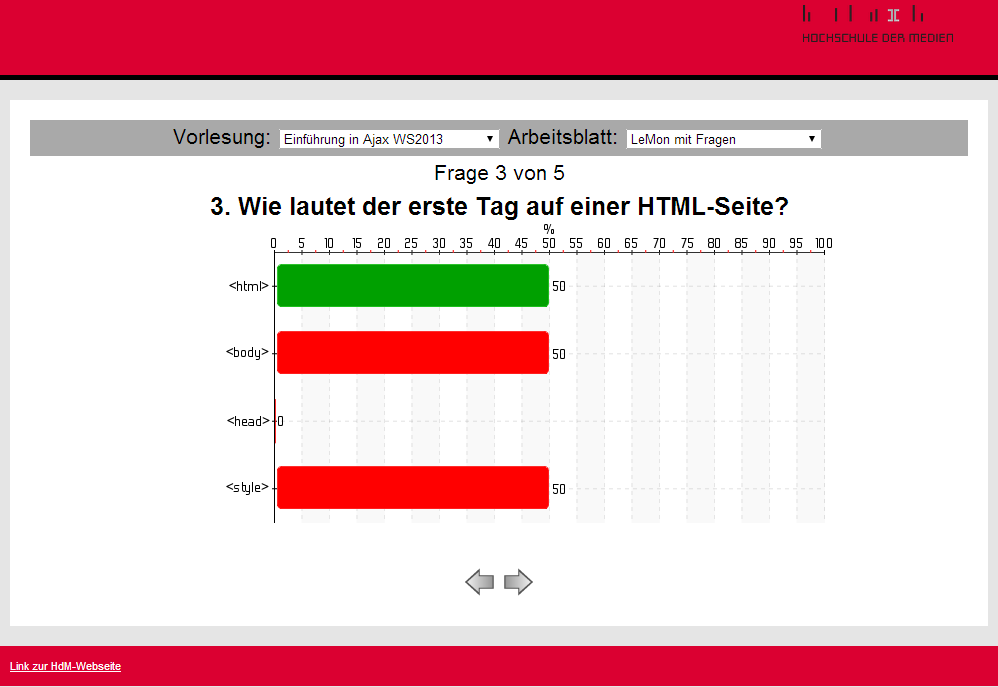
\includegraphics[width=36.6em]{images/Auswertung.png}}\\
 	 	 \end{tabular}
		\caption{Ansicht der Auswertung}
		\label{fig:Auswertung}
	\end{center} 
\end{figure}\FloatBarrier


\chapter{Fazit und Ausblick}

 

% Anhang
\chapter{Anhang} 
\clearpage
\pagenumbering{Roman}

%Glossar ausgeben
\printglossary[ 
	%%style=indexgroup,
	title=Glossar,
	toctitle=Glossar]
    
%   separates Abkürzungsverzeichnis ausgeben  
%   \printglossary[
%   	style=indexgroup,
%   	type=\acronymtype, 
%   	title =Abkürzungsverzeichnis,
%		toctitle=Abkürzungsverzeichnis]

% Abbildungsverzeichnis
\clearpage

%Quellcode-Anhang
%\cleardoublepage
%\phantomsection \label{listofCode}
%\addcontentsline{toc}{section}{Quellcode1}
%\clearpage


\phantomsection \label{listoffig}
\addcontentsline{toc}{section}{Abbildungsverzeichnis}
\listoffigures

%Tabellenverzeichnis
\cleardoublepage
\phantomsection \label{listoftab}
\addcontentsline{toc}{section}{Tabellenverzeichnis}
\listoftables 
 
% Quellcodeverzeichnis
\cleardoublepage
\phantomsection \label{listoflist} 
\addcontentsline{toc}{section}{Quellcodeverzeichnis}
\lstlistoflistings

% im Literaturverzeichnis alles anzeigen, auch die die man nicht verwendet hat 
% \nocite{*} 
% Literaturverzeichnis (durch BibTeX erstellt)

\interlinepenalty=10000 %Seitenumbrüche in einzelnen Einträgen im
% Literaturverzeichnis vermeiden
\bibliography{literaturverzeichnis}{}
\clearpage

% leere Seite am Ende einfügen
%\thispagestyle{empty}
%\textbf{ }
%\cleardoublepage


\end{document} 